\documentclass[11pt]{article}
\usepackage[utf8]{inputenc}
\usepackage[english]{babel}
\usepackage{amsmath}
\usepackage{graphicx}
\usepackage{float}
\usepackage{lipsum}
\usepackage{multicol}
\usepackage{xcolor}
\usepackage{tabularx}
\usepackage{booktabs}
\usepackage{hyperref}
\newcolumntype{Y}{>{\centering\arraybackslash}X}
\usepackage[left=2.00cm, right=2.00cm, top=2.00cm, bottom=2.00cm]{geometry}

\hypersetup{
    colorlinks=true,
    linkcolor=darkgray,
    urlcolor=darkgray,
    citecolor=darkgray,
    pdfborder={0 0 0}
}

\title{AN2DL Reports Template}

\begin{document}
    
    \begin{figure}[H]
        \raggedright
        
\includegraphics[scale=0.4]{reports/images/polimi.png} \hfill 
\includegraphics[scale=0.3]{reports/images/airlab.jpeg}
    \end{figure}
    
    \vspace{5mm}
    
    \begin{center}
        % Select between First and Second
        {\Large \textbf{AN2DL - Second Homework Report}}\\
        \vspace{2mm}
        % Change with your Team Name
        {\Large \textbf{Neural Network November}}\\
        \vspace{2mm}
        % Team Members Information
        {\large Michael Alibeaj,}
        {\large Matteo Bettiati,}
        {\large Lorenzo Bianchi,}
        {\large Francesco Ostidich}\\
        \vspace{2mm}
        % Codabench Nicknames
        {michaelgear01,}
        {betti38,}
        {lollyx21,}
        {francescoostidich}\\
        \vspace{2mm}
        % Matriculation Numbers
        {260044,}
        {258730,}
        {259946,}
        {259863}\\
        \vspace{5mm}
        \today
    \end{center}    
    \vspace{5mm}
    
    \begin{multicols}{2}
        
        \section{Introduction}
        
        In this assignment\cite{lecun2015deep}\cite{polimi_2024_2025} we were provided with grayscale images of Mars terrain, where each pixel is categorized into one of five terrain classes.
        This is a semantic segmentation problem, and our objective was to assign the correct class label to each pixel in the image. 
        To address this challenge, we analyzed the data, built a UNet model, and enhanced its architecture to improve segmentation accuracy.

        \section{Problem Analysis}

        \subsection{Dataset details}
        
        The dataset consists of 64x128 grayscale images (1 channel).
        There are five classes: 0 for \textit{background}, 1 for \textit{soil}, 2 for \textit{bedrock}, 3 for \textit{sand}, and 4 for \textit{big rock}.
        The training set (comprehending images and labels) is an array of shape (2615, 2, 64, 128), the test set is instead an array of shape (10022, 64, 128) of unlabeled images.
        
        \subsection{Main challenges}
        
        Several challenges arose during this task.
        Firstly, the small image size limits the detail level, thus blurring class boundaries with varying terrain types.
        Class imbalance, with the \textit{background} class dominating, hurted performance for underrepresented classes, i.e. \textit{big rock}. 
        Lastly, more generally, the Mars terrain complexity and irregular textures further complicated the model ability to generalize.
        
        \section{Methods}

        \subsection{Exploratory data analysis}
        
        During the EDA phase, a grid of sample images along with their respective masks was plotted.
        This visualization helped identify a series of outliers, referred to as "aliens".
        These outliers were removed by leveraging the associated masks, which were identical across all identified outliers. 
        The class distribution was then analyzed, revealing that class 4 was severely underrepresented
        
        \subsection{Data augmentation}
        
        To increase dataset diversity and improve generalization, we tried to apply random rotations, flips, scaling, cut mix, blur, elastic deformations, brightness and contrast to the images. 
        Different combinations of functions made the model perform differently: the augmentation pipeline has thus been taylored ad hoc, based on the best metrics we observed when training the models.
        In the end, to address the class imbalance, images containing class 4 were duplicated multiple times (approximately 15 to 20 times) until a more balanced dataset was achieved.
        The main augmentation fuction we used in the end was cut mix, which created new samples by pasting patches from 2 to 4 other samples onto the existing images. 
        This technique increased the dataset size to around 10,000 samples.
        To ensure robust model performance evaluation, the validation split was also augmented.
        Finally, the entire dataset was fed into the model through a data loader, which dynamically applied simple augmentations such as flipping and rotations during training.
        Augmentations helped the model handle variations in terrain orientation and spatial configuration.
        
        \subsection{UNet architecture}
        
        The model we used was a custom UNet model, utilizing an encoder-decoder structure with skip connections to preserve spatial information. 
        This architecture enabled the model to extract hierarchical features and make pixel-wise predictions. 
        The training we made was made almost every time on the augmented dataset.

        \begin{figure}[H]
            \centering
            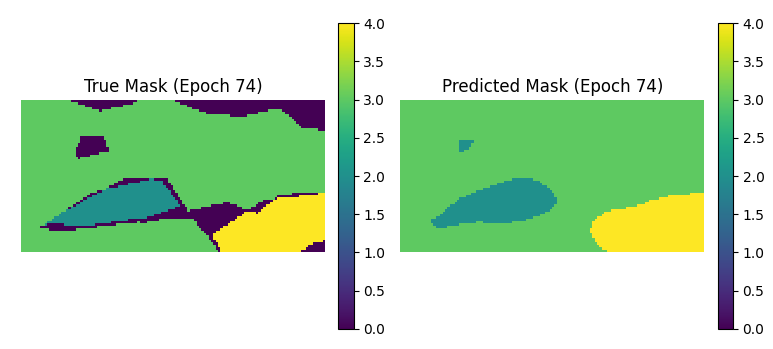
\includegraphics[width=0.45\textwidth]{reports/images/prediction1.png}
            \caption{\small Mid-training prediction}
        \end{figure}
        
        \subsection{Loss function exploration}
        
        We experimented with various loss functions during the training phase.
        We started with a \textit{categorical cross-entropy}, for later exploring a \textit{dice loss} and a {mean intersection over union loss}.
        Moreover, we also opted for combining losses together hoping to find better compromises and therefore better results.
        In the end, the \textit{focal loss} was the best scoring alternative; we also exploited the \textit{class weights} implementation of this loss function, which massively helped the model focus on smaller classes like {big rock} and improve both global and local segmentation accuracy.
        
        \section{Experiments}
        
        \subsection{Model architecture adjustments}
        
        The layers of out UNet model architecture were fine tuned during the training process.
        By adjusting the number of convolutional layers, filter sizes, and kernel depths, feature extraction improved, and pixel-wise predictions got more distincts.
        These adjustments helped the model capture more complex terrain features.

        Training was conducted on Colab\cite{colab2024} and Kaggle\cite{kaggle2024} GPUs
        The TensorFlow\cite{tensorflow2015} Keras\cite{keras2015} and PyTorch\cite{pytorch2019} frameworks were also utilized during model development and training.
        
        \subsection{Advanced architectures}
        
        We also explored more advanced architectures.
        One of those was a dual UNet model, which combined outputs from two parallel UNets.
        Others were transformers architectures, which managed to capture long-range dependencies.
        Additionally, we also incorporated residual blocks to improve gradient flow and prevent overfitting, enhancing the model learning capacity.

        \section{Conclusions}
        
        \subsection{Contribution}

        Experimentation and training tasks were carried out equally and coordinately by each team member.
        Everyone mainly focused on a specific objective, as follows.
        Alibeaj worked on the development and implementation of the UNet architecture.
        Bettiati focused on refining and optimizing the UNet model for better performance.
        Bianchi investigated and experimented with various loss functions to improve segmentation accuracy.
        Ostidich led the data augmentation efforts, applying various transformations to enhance model generalization.

        \bibliographystyle{abbrv}
        \bibliography{reports/references}

    \end{multicols}
\end{document}